
\chapter{The toric code}

\section{Decoders}
\subsection{The optimal decoder}
\subsection{Minimum Weight Perfect Matching}
\subsection{The Union-Find decoder}

Even the fastest MWPM algorithms still have a quadratic time complexity of $\mathcal{O}(n^2\sqrt{n})$, where $n$ is the number of qubits. In order to realistically utilize a decoder with increasing decoding success rates using increasing lattice size, we would need to have a better time complexity. Luckily, an alternative algorithm called the Peeling Decoder has been developed which can solve errors over the erasure channel with a linear time complexity $\mathcal{O}(n)$ \cite{delfosse2017}. The Union-Find Decoder builds on top of the Peeling Decoder to solve for Pauli errors with a time complexity of $\mathcal{O}(n\alpha(n))$, where $\alpha$ is an inverse Ackermann function, which is smaller than 3 for any practical input size \cite{nickerson2017}. However, these algorithms have a tradeoff in the form of a decrease in the error threshold, and has the reported value of $p_{UF} = 9.2\%$.

A topic of interest will be weighted growth function for the Union-find decoder. This function of the algorithm will increase the error threshold to $p_{UF} = 9.9\%$, but has not been fully described in its publication.  In this section, we will describe the original Peeling decoder and the Union-Find decoder.   \\

\subsubsection{The Peeling decoder}
Let $\varepsilon \subset E$ be an erasure, a set of qubits on which an erasure error occurs, and let $\sigma \subset S$ be the measured error syndrome, the subset of stabilizer generators which anticommute with the erasure errors. In the absence of Pauli errors, all errors $P$ must lie inside the erasure. Therefore, for any pair of stabilizer generators in $\sigma$, the path of errors must also be in the erasure, which can be denoted by $P\subset \varepsilon$. Furthermore, due to the fact that errors $P$ are randomly distributed, any coset of errors and stabilizers $P\cdot S$ that solves the error syndrome $\sigma$ is the most likely coset. These features of an erasures forms the basis of the Peeling decoder. In order to find a coset of $P \cdot S$, the decoder reduces the size of the erasure by peeling edges from the erasure, while keeping the syndromes at the new boundary of the erasure. Elements of the syndrome can be moved by applying an correction on the adjacent qubit. At the end, the entire erasure is peeled or removed, and all corrections will have removed the errors up to a stabilizer.

\tikzset{
  anyon/.style={circle, fill=OrangeRed, minimum size=.2cm, inner sep=0},
  erasure/.style={NavyBlue, very thick},
  correction/.style={Green, very thick},
  description/.style={align=#1, anchor=west, text width=4cm},
  description/.default={left},
  error/.style={text=black, pos=0.5}
  }

\begin{figure}
  \centering
  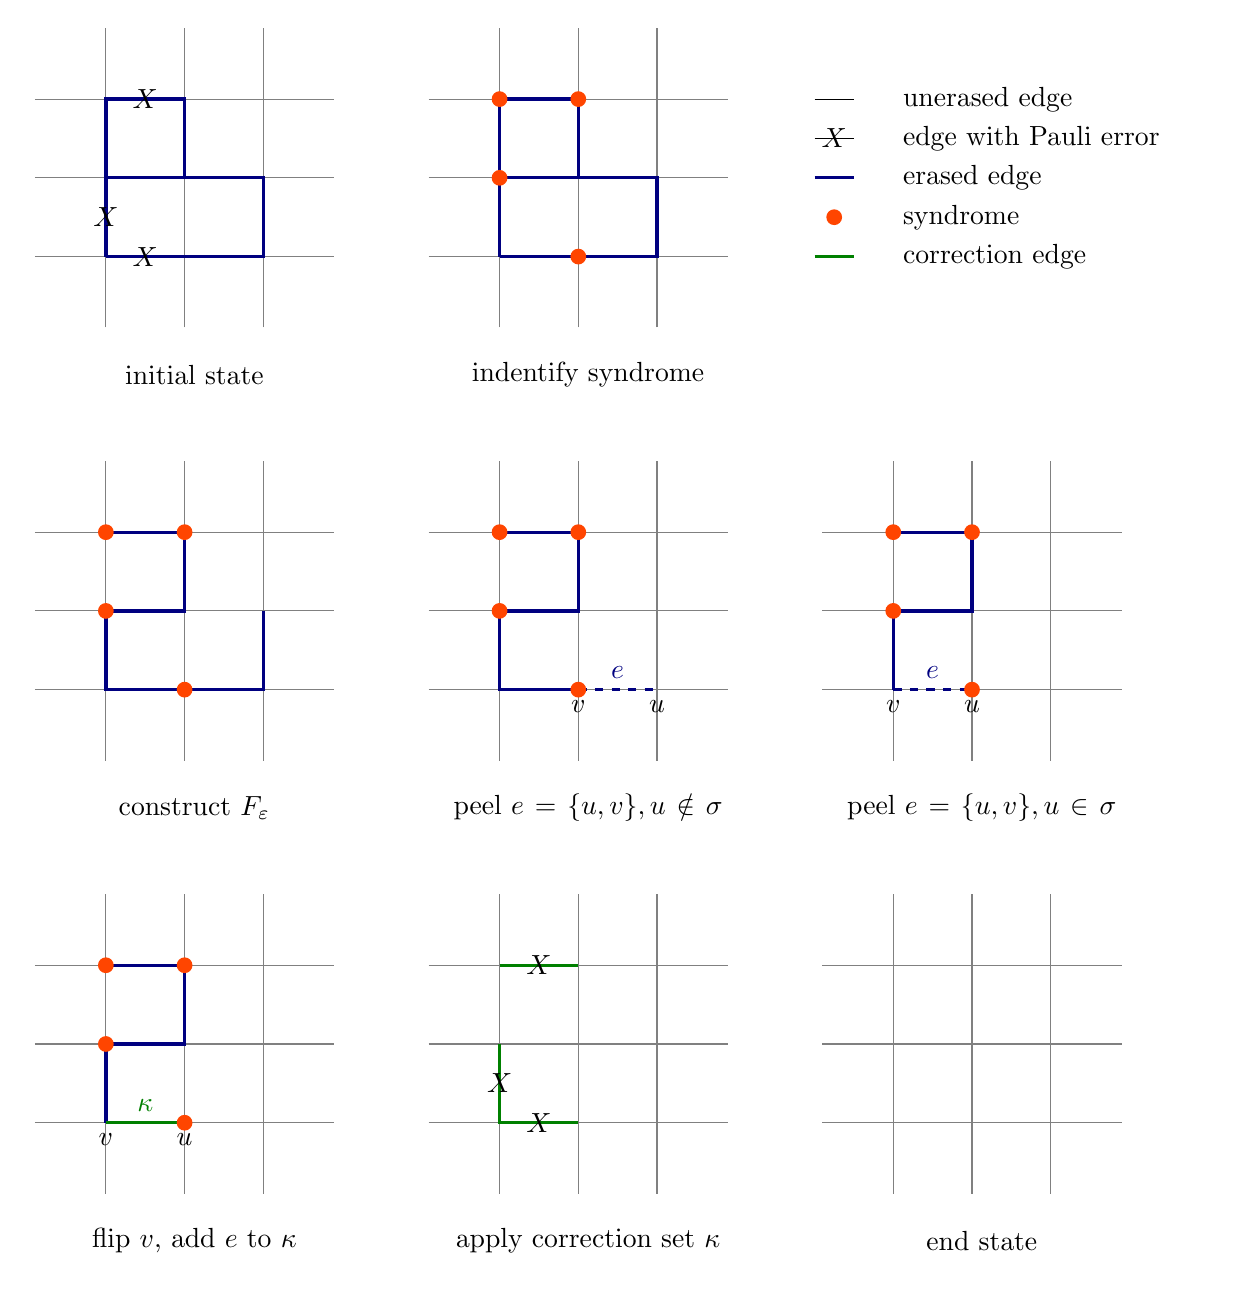
\begin{tikzpicture}
   
    \draw[step=1cm,gray,thin] (0.1,0.1) grid (3.9,3.9);
    \draw[erasure] (1,1) -- (2,1) node[error]{$X$} -- (3,1) -- (3,2) -- (2,2) -- (1,2) -- (1,1) node[error]{$X$};
    \draw[erasure] (1,2) -- (1,3) -- (2,3) node[error]{$X$} -- (2,2);
    \node[description={center}] at (0, -.5) {initial state};
    
    \begin{scope}[shift={(5,0)}]
      \draw[step=1cm,gray,thin] (0.1,0.1) grid (3.9,3.9);
      \draw[erasure] (1,1) -- (2,1) -- (3,1) -- (3,2) -- (2,2) -- (1,2) -- (1,1);
      \draw[erasure] (1,2) -- (1,3) -- (2,3) -- (2,2);
      \node[anyon] at (1,2) {};
      \node[anyon] at (2,1) {};
      \node[anyon] at (1,3) {};
      \node[anyon] at (2,3) {};
      \node[description={center}] at (0, -.5) {indentify syndrome};
    \end{scope}
    
    \begin{scope}[shift={(10,1)}]
      \draw[thin] (0,2) -- (.5,2) ;
      \node[description] at (1, 2) {unerased edge};
      \draw[thin] (0,1.5) -- (.5,1.5)  node[error]{$X$};
      \node[description] at (1, 1.5) {edge with Pauli error};
      \draw[erasure] (0, 1) -- (.5, 1);
      \node[description] at (1, 1) {erased edge};
      \node[anyon] at (0.25, .5) {};
      \node[description] at (1, .5) {syndrome};
      \draw[correction] (0,0) -- (.5,0);
      \node[description] at (1, 0) {correction edge};
    \end{scope}
    
    \begin{scope}[shift={(0,-5.5)}]
      \draw[step=1cm,gray,thin] (0.1,0.1) grid (3.9,3.9);
      \draw[erasure] (1,3) -- (2,3) --  (2,2) -- (1,2) -- (1,1) -- (2,1) -- (3,1) -- (3,2);
      \node[description={center}] at (0, -.5) {construct $F_{\varepsilon}$};
      \node[anyon] at (1,2) {};
      \node[anyon] at (2,1) {};
      \node[anyon] at (1,3) {};
      \node[anyon] at (2,3) {};
    \end{scope}
    
    \begin{scope}[shift={(5,-5.5)}]
      \draw[step=1cm,gray,thin] (0.1,0.1) grid (3.9,3.9);
      \draw[erasure] (1,3) -- (2,3)  --  (2,2) -- (1,2) -- (1,1) -- (2,1);
      \draw[erasure, dashed] (2,1) -- (3,1) node[pos=0, below, text=black]{$v$} node[pos=0.5, above]{$e$} node[pos=1, below, text=black]{$u$};
      \node[description={center}] at (0, -.5) {peel $e=\{u,v\}, u \notin \sigma$};
      \node[anyon] at (1,2) {};
      \node[anyon] at (2,1) {};
      \node[anyon] at (1,3) {};
      \node[anyon] at (2,3) {};
    \end{scope}
    
    \begin{scope}[shift={(10,-5.5)}]
      \draw[step=1cm,gray,thin] (0.1,0.1) grid (3.9,3.9);
      \draw[erasure] (1,3) -- (2,3)  --  (2,2) -- (1,2) -- (1,1);
      \draw[erasure, dashed] (1,1) -- (2,1) node[pos=0, below, text=black]{$v$} node[pos=0.5, above]{$e$} node[pos=1, below, text=black]{$u$};
      \node[description={center}] at (0, -.5) {peel $e=\{u,v\}, u \in \sigma$};
      \node[anyon] at (1,2) {};
      \node[anyon] at (2,1) {};
      \node[anyon] at (1,3) {};
      \node[anyon] at (2,3) {};
    \end{scope}
   
    \begin{scope}[shift={(0,-11)}]
      \draw[step=1cm,gray,thin] (0.1,0.1) grid (3.9,3.9);
      \draw[erasure] (1,3) -- (2,3)  --  (2,2) -- (1,2) -- (1,1);
      \draw[correction] (1,1) -- (2,1) node[pos=0, below, text=black]{$v$} node[pos=0.5, above]{$\kappa$} node[pos=1, below, text=black]{$u$};
      \node[description={center}] at (0, -.5) {flip $v$, add $e$ to $\kappa$};
      \node[anyon] at (1,2) {};
      \node[anyon] at (2,1) {};
      \node[anyon] at (1,3) {};
      \node[anyon] at (2,3) {};
    \end{scope}
    
    \begin{scope}[shift={(5,-11)}]
      \draw[step=1cm,gray,thin] (0.1,0.1) grid (3.9,3.9);
      \draw[correction] (1,3) -- (2,3) node[error]{$X$};
      \draw[correction] (2,1) -- (1,1) node[error]{$X$} -- (1,2) node[error]{$X$};
      \node[description={center}] at (0, -.5) {apply correction set $\kappa$};
    \end{scope}
    
    \begin{scope}[shift={(10,-11)}]
      \draw[step=1cm,gray,thin] (0.1,0.1) grid (3.9,3.9);
      \node[description={center}] at (0, -.5) {end state};
    \end{scope}
  \end{tikzpicture}
  \caption{Schematic representation of the Peeling decoder.}
\end{figure}

We will now describe the Peeling decoder as is presented in Algorithm \ref{algo:peel}. In step 1, we will remove all cycles present in $\varepsilon$. We construct a spanning forest $F_\varepsilon$ inside erasure $\varepsilon$, the maximal subsect of edges of $\varepsilon$ that contains no cycles and spans all vertices of $\varepsilon$. From here, we loop over all edges in $F_\varepsilon$ (step 3), starting at a leaf edge $e = \{u,v\}$, removing the leaf edge from $F_\varepsilon$ (step 4), and conditionally add the edge to the correction set $\kappa$ if the pendant vertex $u$ is in $\sigma$ (step 6). If the correction is applied immediately, we can see that the pendant vertex $u$ is removed from $\sigma$ and that the value of $v$ is flipped in $\sigma$. Edges on a branch in the forest will be added to $\kappa$ until $v \in \sigma$, or a generator will be continuously moved from $u$ to $v$ until it encounters another generator, creating a correction path between two syndrome pairs.

\begin{algo}[algotitle=Peeling decoder \cite{delfosse2017}, label=algo:peel]
\begin{algorithm}[H]
    \SetAlgoNoEnd
    \KwData{A graph $G = (V,E)$, an erasure $\varepsilon \subset E$ and syndrome $\sigma \subset V$}
    \KwResult{Correction set $\kappa \subset E$}
    \BlankLine
    construct a spanning forest $F_\varepsilon$ of $\varepsilon$\;
    initialize $\kappa$ by $\kappa = {\O}$\;
    \While{$F_\varepsilon \neq \O$}{
        pick a leaf edge $e = {u,v}$ with pendant vertex $u$, remove $e$ from $F_\varepsilon$ \;
        \If{$u \in \sigma$}{
            add $e$ to $\kappa$, remove $u$ from $\sigma$ and flip $v$ in $\sigma$}
        \Else{do nothing}
    }
    \KwRet{$\kappa$}
\end{algorithm}
\end{algo}

\noindent Note that due the flipping of both $u$ and $v$ in $\sigma$, the parity of the number of generators in $\sigma$ is always preserved. The peeling decoder can therefore always solve erasures with an even parity, as the size of $\sigma$ will drop until at the end the syndrome will be empty $\sigma = \O$, and call errors are corrected up to a stabilizer. This is always the case in the absence of measurement and Pauli errors, as all errors within the erasure either add or remove an even number of generators to or from $\sigma$.

\paragraph{Time complexity of the Peeling decoder}
The spanning forest $F_\varepsilon$ can be constructed in linear time. Also, the loop over the forest can be operated in linear if the list of leaves is pre-computed and updated during the loop. Thus the Peeling decoder has a linear time complexity in the size of the erasure $\mathcal{O}(\abs{\varepsilon})$ and therefore also in the number of qubits $\mathcal{O}(n)$.

\subsubsection{Growing erasures}

Now in the presence of Pauli errors, errors can occur on edges that are now not part of the erasure, and odd parity clusters can occur. Clusters that consists from only a single generator also exist, which are just end-points of syndromes caused by Pauli errors. We must therefore make an erasure $\varepsilon$ from the syndrome $\sigma$ that is compatible with the peeling decoder, which contains only even parity clusters. To do this, we can iteratively grow the clusters with an odd parity by an half-edge on the boundaries on the clusters. When two odd parity clusters meet, the merged cluster will have a even parity, and can now be solved by the peeling decoder.

\paragraph{Union-Find algorithm}

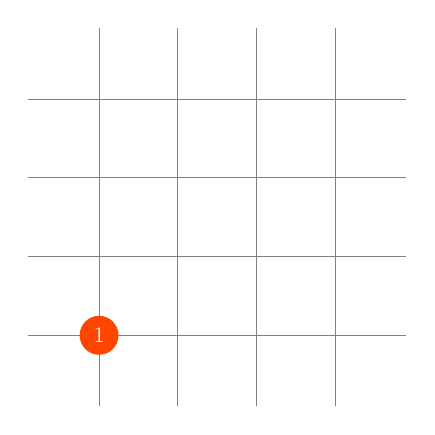
\begin{tikzpicture}
  \draw[step=1cm,gray,thin] (0.1,0.1) grid (4.9, 4.9);
  \node[fill=OrangeRed, circle, text=white, scale=0.8] (N0) at (1, 1) {1};

\end{tikzpicture}

To keep track of the vertices of a cluster, it will be represented as a \emph{cluster tree}, where an arbitrary vertex of the cluster will be the root, and any other vertex will be a child of the root. Whenever an edge $(u,v)$ is fully grown, we will need to traverse the trees of the two vertices $u$ and $v$, and check wether they have the same root; whether they belong to the same cluster. If not, a merge is initiated by making the root of smaller cluster a child of the bigger cluster. These functions, \codefunc{find} and \codefunc{union} respectively, are part of the Union-Find algorithm (not to be confused with the Union-Find decoder) \cite{tarjan}.

\begin{tikzpicture}
  \draw (2,2) circle (0.2);
  \draw (2,2) -- (0,0);)
\end{tikzpicture}

Within the Union-Find algorithm, two features ensure that the complexity of the algorithm is not quadratic. 1). With \textbf{path compression}, as we traverse a tree from child to parent until we reach the root, we make sure that each vertex encountered that we have encountered along the way is pointed directly to the root. This doubles the cost of the \codefunc{find}, but speeds up any future call to any vertex on the traversed path. 2). With \textbf{weighted union}, we make sure to always make the smaller tree a child of the bigger tree. This ensures that the overall length of the path to the root stays minimal. In order to make this happen, we just need to store the size of the tree at the root.

\paragraph{Data structure}
Now it is clear what information is exactly needed to grow the clusters using the Union-Find algorithm. We will need to store the cluster in a sort of cluster-tree. At the root of each tree we store the size and parity of that cluster in order to facilitate weighted union and to select the odd clusters. We will need to store the state of each edge (empty, half-grown, or fully grown) in a table called \codeword{support}. And we need to keep track of the boundary of each cluster in a \codeword{boundary} list.

\paragraph{The routine}
The full routine of the Union-Find decoder as originally described (\cite{nickerson2017}, Algorithm 2) is listed in Algorithm \ref{algo:uf}. In line 1-2, we initialize the data structures, and a list of odd cluster roots $\mathcal{L}$. We will loop over this list until it is empty, or that there are no more odd clusters left.

In each growth iteration, we will need to keep track of which clusters have merged onto one, therefore the fusion list $\mathcal{F}$ is initialized in line 4. We loop over all the edges from the \codeword{boundary} of the clusters from $\mathcal{L}$ in line 5, and grow each edge by an half-edge in \codeword{support}. If an edge is fully grown, it is added to $\mathcal{F}$.

For each edge $(u,v)$ in $\mathcal{F}$, we need to check whether the neighboring vertices belong to different clusters, and merge these clusters if they do. This is done using the Union-Find algorithm in line 6. We call \codefunc{find(u)} and \codefunc{find(v)} to find the cluster roots of the vertices. If they do not have the same root, we make one cluster the child of another by \codefunc{union(u,v)}. Note that this does not only merge two existing clusters, also new vertices, which have themselves as their roots, are added to the cluster this way. We also need to combine the boundary lists of the two clusters.

Finally, we need to update the elements in the cluster list $\mathcal{L}$. First, we replace each element $u$ with its potential new cluster root \codefunc{find(u)} in line 7. We can avoid creating duplicate elements by maintaining an extra look-up table that keeps track of the elements $\mathcal{L}$ at the beginning of each round of growth. In line 8, we update the \codeword{boundary} lists of all the clusters in $\mathcal{L}$, and in line 9, even clusters are removed from the list, preparing it for the next round of growth.

\begin{algo}[algotitle=Union-Find decoder \cite{nickerson2017}, label=algo:uf]
\begin{algorithm}[H]
    \SetAlgoNoEnd
    \KwData{A graph $G = (V,E)$, an erasure $\varepsilon \subset E$ and syndrome $\sigma \subset V$}
    \KwResult{A grown erasure $\varepsilon'$ such that each cluster $\gamma \subset \varepsilon$ is even}
    \BlankLine
    initialize cluster-trees, support and boundary lists for all clusters \;
    initialize list of odd cluster roots $\mathcal{L}$\;
    \While{$\mathcal{L} \neq \emptyset$}{
      initialize fusion list $\mathcal{F}$ \;
      for all $u \in \mathcal{L}$, grow all edges in the boundary list of cluster $C_u$ by a half-edge in support. If the edge is fully grow, add to fusion list $\mathcal{F}$ \;
      for all $e={u,v} \in \mathcal{F}$, if \emph{find($u$)} $\neq$ \emph{find($v$)}, then apply \emph{union($u,v$)}, append boundary list\;
      for all $u \in \mathcal{L}$, replace $u$ with \emph{find($u$)} without creating duplicate elements\;
      for all $u \in \mathcal{L}$, update the boundary list\;
      remove even clusters from $\mathcal{L}$\;
    }
    run peeling decoder with grown erasure $\varepsilon'$
\end{algorithm}
\end{algo}

\subsubsection{Time complexity of the Union-Find decoder}

\subsection{Finding clusters}

\subsection{Bucket Cluster Sort}
To further increase the error threshold for the Union-Find decoder from $9.2\%$ to $9.9\%$, Nickerson implements weighted growth, where clusters are grown in increasing order based on their sizes \cite{delfosse2017}. However, the main problem with weighted growth is that the clusters now need to be sorted, and that after each growth iteration another round of sorting is necessary, due to the fact that the clusters have changed sizes due to growth and merges, and the order of clusters may have been changed. Nickerson has not given a description of how weighted growth in implemented. From a review of the Union-Find decoder, an implementation of weighted growth is described using \emph{Heapsort}, which has been incorrectly described as linear as its time complexity is also $\mathcal{O}(n\log(n))$ \cite{nando}. As the complexity of the algorithm is now dominated by the Union-Find algorithm, we need to make sure that weighted growth does not add to this complexity. To avoid this iterative sorting, we need to make sure that the insertion of a new element in our sorted list of clusters does not depend on the values in that list.

The Bucket Cluster sorting algorithm as described in this section is evolved from a more complicated version that is described in appendix \ref{ap.bucketsort}, which has a sub-linear complexity of $\mathcal{O}(\sqrt{n})$.

\subsubsection{How to sort for weighted growth}

Let us now first look at what weighted growth for the Union-Find decoder exactly does. When a cluster is odd, there exists at least one path of errors connecting this cluster to a generator outside of this cluster. When the cluster grows, a number of edges $k$ that is proportional to the size of the cluster $S$ is added to the cluster. If $k \propto S$ new edges are added, only $1/k$ of these edges will correctly connect the cluster with the generator. Therefore, more "incorrect" edges will be added during growth of a larger cluster.

Note however, that the benefit of growing a smaller cluster is not substantial if the clusters are of similar size. Take two clusters with size $S_A <<S_B$, growth of cluster B will add $\sim k_B/2$ "incorrect" edges on average, whereas growth of cluster A will add $\sim k_A/2 << k_B/2$ edges as $k_A \propto S_A$ and $k_B \propto S_B$. However, if $S_A \simeq S_B$, the number of added "incorrect" edges for both clusters will also be similar, and it is the same when $S_A = S_B$. Thus clusters with the same size can be grown "simultaneously", as there is no benefit to grow one before another.

\begin{lemma}
  Weighted growth of cluster A with size $S_A << S_B$ ensures that a smaller amount of "incorrect" edges is added, compared with growth of cluster B.
\end{lemma}

The sorting method that is suited for our case is \emph{Bucket sort}. In this algorithm, the elements are distributed into $k$ buckets, after which each bucket is sorted individually and the buckets are concatenated to return the sorted elements. Applied to the clusters, we sort the odd-parity clusters into $k$ buckets. As the sizes of the clusters can only take on integer values, each bucket can be assigned a clusters size, and sorting of each individual bucket is not necessary. Furthermore, as we are not interested in the overall order of clusters, concatenating of the buckets is not necessary.

\paragraph{Growing a bucket}
The procedure for the Union-Find decoder using the bucket sort algorithm is now to sequentially grow the clusters from a bucket starting from bucket 0, which contain the smallest single-generator clusters of size 1. After a round of growth, in the case of no merge event, these clusters are grown half edges, but are still size 1. We would therefore need twice as many buckets to differentiate between clusters without and with half-edges. Let us call them full-edged and half-edged clusters, respectively. Starting from bucket 0, even buckets contain full-edged clusters and odd buckets contain half-edged clusters of the same size. To grow a bucket, clusters are popped from the bucket, grown on the boundary, after which the clusters is to be distributed in a bucket again. In the case of no merge event, clusters grown from even bucket $i$ must be placed in odd bucket $i + 1$, as it does not increase in size, and clusters grown from odd bucket $j$ must be placed in even bucket $j + 2k + 1$ with $k \in \mathbb{N}_0$. Also in the case of a merge event of clusters A and B, the new cluster AB must be placed in a bucket $i_{AB} > i_A, i_{AB} > i_B$. Thus we can grow the buckets sequentially, and need not to worry about bucket that have been already "emptied".
\begin{lemma}
  Buckets can be grown sequentially after each other as new clusters will always be placed in a higher bucket than the current one.
\end{lemma}

\paragraph{Faulty entries}

\begin{figure}
  \centering
  \includegraphics[width=\linewidth]{cluster_merge_A.pdf}
  \caption{Faulty entries of clusters can occur in the buckets, a) cluster that should not be there due to a merge event. Situation a can be solved by checking the parity of the cluster. Checking the parity of the root cluster solves a) and b). Checking the bucket\_number of the root cluster solves all.}\label{3.fig.clustermergeB}
\end{figure}

Now let us be clear: \emph{only odd parity clusters will be placed in buckets, but each bucket does not only contain odd parity clusters}. As a merge happens between two odd parity clusters A and B during growth of B, cluster A has already been placed in a bucket, as it was still odd after its growth. But cluster A is now part of cluster AB and has even parity, and the entry of cluster A is faulty. To prevent growth of the \emph{faulty entry}, we can check for the parity of the root cluster.

Furthermore, it is possible that another cluster C merges onto AB, such that the cluster ABC is odd again. Now, the faulty entry of cluster A passes the previous test. To solve this issue, we store an extra \codeword{bucket_number} at the root of a cluster. Whenever a cluster increases in size or merges to an odd parity cluster, we first update the \codeword{bucket_number} to the appropriate value and place it in its bucket. If the cluster merges to an even parity cluster, we update the \codeword{bucket_number} to \codeword{None}. Now, every time a cluster is popped from bucket $i$, we can just check weather the current bucket corresponds to the \codeword{bucket_number} of the root cluster.

\paragraph{Number of buckets}
How many buckets do we exactly need? On a lattice there can be $n$ vertices, and a clusters can therefore grow to size $n$, spanning the entire lattice. Naturally, if a cluster spans the entire lattice, the solution given by the peeling decoder is now trivial. But we need to make sure that the decoder \emph{can} give a solution. As we are only placing odd parity clusters in buckets, and clusters of the same size grow "simultaneously", the largest odd parity cluster should only cover about half the lattice, while another odd parity cluster of the same size covers the other half. Any odd parity cluster that is larger than that should now grow as there should always be a smaller cluster available to grow instead. We can show that the largest odd parity cluster size is $S_M = L\times(\lfloor L/2\rfloor - 1)$ with $L=\sqrt{n}$ on a square lattice. This results to $N_b = 2L\times(\lfloor L/2\rfloor - 1)$ buckets. Any odd parity cluster with bucket number larger $N_b$ shall be assigned \codeword{bucket_number=None} and will not be placed in a bucket, as there is no bucket available.

\paragraph{Largest bucket occurrence}
Not all buckets will be filled depending on the configuration of the lattice. It would therefore be redundant to go through all buckets just to find out that the majority of them is empty. To combat this, we can keep track of the largest bucket occurrence $i_{M,o}$. Whenever a bucket $i$ has been emptied and $i = i_{M,o}$, we can break out of the bucket loop to skip the remainder of the buckets.

\subsubsection{Complexity}
Let us focus on the operations on a single cluster before it is grown an half-edge. A cluster is placed in a bucket, popped from that bucket some time after, checked for faulty entry, and if passed grown. All these operations are done linear time $\mathcal{O}(1)$. There are a maximum of $\mathcal{O}(L^2) = \mathcal{O}(n)$ buckets to go through. Thus the overall complexity of $\mathcal{O}(n\alpha(N))$ is preserved.

\subsubsection{The Bucket Union-Find decoder}


\subsection{Object oriented approach}

Others who have implemented weighted growth (wrongly) use an algorithm that has a time complexity of $\mathcal{O}(n\log n)$, which is worse than the main algorithm \cite{nando}. We will introduce a weighted growth algorithm that has a linear time complexity, and therefore preserving the inverse Ackermann time complexity of the Union-Find decoder.

\subsubsection{A new data structure}

\subsubsection{Parent-child method for merging boundary lists}

\begin{figure}
  \centering
  \includegraphics[width=\linewidth]{parent_child_A.pdf}
  \caption{The parent-child method for merging boundary lists. By storing a list of pointers of child clusters at the parent cluster, we needn't append the full boundary list from the child to the parent cluster. The tree representation (TR) is shown on the top right. } \label{3.fig.parentchildA}
\end{figure}

When two clusters merge, one needs to check for the larger cluster between the two, and make the smaller cluster the child of the bigger cluster, which lowers the depth of the tree and is called the \emph{weighted union rule}. Applied to the toric lattice, the Union-Find decoder also needs to append the boundary list (which contains all the boundary edges of a cluster) of the smaller cluster onto the list of the larger cluster. This method, as explained before, requires that the new boundary list needs to be checked again.

In our application, instead of appending the entire boundary list, we just add a pointer stored at the parent cluster to the child cluster. As a parent can have many children, the pointers are appended to a list \codeword{children}. When growing a cluster, we first check if this cluster has any child clusters. If yes, these child clusters will be grown first by popping them from the list, but any new vertices will always be added to the parent cluster. Also during and after a merge, we make sure that any new vertices are always added to the parent cluster. Any child will exist in the list of a parent for one round of growth, after which its boundaries will be grown, and the child is absorbed into the parent. This method also works recursively by keeping track of the root cluster instead of just the parent cluster, and many levels of parent-child relationships can exists, but again, only for one round of growth.

\begin{figure}
  \centering
  \includegraphics[width=\linewidth]{parent_child_B.pdf}
  \caption{Growing a merged boundary using the parent-child method. The tree representation (TR) is shown on the top right. }\label{3.fig.parentchildB}
\end{figure}









